%% packages
\documentclass{article}
\usepackage[a4paper, left=2.0cm, right=2.0cm, top=3.5cm]{geometry}
\usepackage[ngerman]{babel}
\usepackage{graphicx}
\usepackage{multicol}
\usepackage{amssymb}
\usepackage{titlesec}
\usepackage{wrapfig}
\usepackage{blindtext}
\usepackage{lipsum}
\usepackage{caption}
\usepackage{listings}
\usepackage{fancyhdr}
\usepackage{nopageno}
\usepackage{authblk}
\usepackage{amsmath} % tons of math stuff
\usepackage{mathtools} % e.g. alignment within matrix
%\usepackage{bm} % provides shorthand for bold in math mode
\usepackage{dsfont} % \mathds makes double stroke digits
\usepackage{esdiff} % provides \diff
%\usepackage[ISO]{diffcoeff}
\usepackage{xcolor}
\usepackage{csquotes} % e.g. provides \enquote
\usepackage[separate-uncertainty=true]{siunitx} % units
\usepackage{xcolor} % colored text
\usepackage[l3]{csvsimple}
\usepackage{subcaption}
\usepackage{physics}
\usepackage{hyperref}
\usepackage{nameref}
\hypersetup{colorlinks=true, linkcolor=black, pdfhighlight={/N}}
\usepackage{tcolorbox}
\usepackage{amsthm}
\usepackage{gensymb} % add \degree in math mode?
\usepackage{newunicodechar} % define custom unicode characters
\usepackage{booktabs}
\usepackage{subcaption}

% \sisetup{
%   scientific-notation = auto,  % Automatically use scientific notation for large/small numbers
%   output-exponent-marker = \text{e}  % (optional) for formatting the exponent symbol
% }



%\fancyhf[]{}

%% custom stuff
% own units
\DeclareSIUnit \VSS {\ensuremath{V_\mathrm{SS}}}
\DeclareSIUnit \VS {\ensuremath{V_\mathrm{S}}}
\DeclareSIUnit \Veff {\ensuremath{V_\mathrm{eff}}}
\DeclareSIUnit \Vpp {\ensuremath{V_\mathrm{pp}}}
\DeclareSIUnit \Vp {\ensuremath{V_\mathrm{p}}}
\DeclareSIUnit \VRMS {\ensuremath{V_\mathrm{RMS}}}
\DeclareSIUnit \ASS {\ensuremath{A_\mathrm{SS}}}
\DeclareSIUnit \AS {\ensuremath{A_\mathrm{S}}}
\DeclareSIUnit \Aeff {\ensuremath{A_\mathrm{eff}}}
\DeclareSIUnit \App {\ensuremath{A_\mathrm{pp}}}
\DeclareSIUnit \Ap {\ensuremath{A_\mathrm{p}}}
\DeclareSIUnit \ARMS {\ensuremath{A_\mathrm{RMS}}}

% change subsection numbering to capital letters
\newcommand{\subsectionAlph}{ \renewcommand{\thesubsection}{\arabic{section}.\Alph{subsection}} }
% change subsection numbering to lowercase letters
\newcommand{\subsectionalph}{ \renewcommand{\thesubsection}{\arabic{section}.\alph{subsection}} }
% change subsubsection numbering to lowercase letters
\newcommand{\subsubsectionalph}{ \renewcommand{\thesubsubsection}{\arabic{section}.\arabic{subsection}.\alph{subsubsection}} }
% own fig. that works with multicols
\newenvironment{Figure}
  {\par\medskip\noindent\minipage{\linewidth}}
  {\endminipage\par\medskip}
\newcommand*{\inputPath}{./plot} % prepend this command to the argument of all input commands
\graphicspath{ {./images/}{./figure/}{../plot/}{../../plot/}{../../latex/assets/}{./assets/} }
% own enviroment for definitions
\newenvironment{definition}[1]
{\begin{quote} \noindent \textbf{\textit{#1\ifx&#1& \else : \fi}} \itshape}
{\end{quote}}

\newunicodechar{°}{\degree}


% own commands
% \newcommand{\rarr}{$\to\,$} %A$\,\to\,$B
\newcommand{\defc}{black}
\newcommand{\colorT}[2][blue]{\color{#1}{#2}\color{\defc}}
\newcommand{\redq}{\color{red}(?)\color{\defc}}
\newcommand{\question}[1]{\colorT[purple]{\textbf{(#1)}}}
\newcommand{\todo}[1]{\colorT[red]{\textbf{(#1)}}}
\newcommand{\mr}{\mathrm}

%% preparation
\begin{titlepage}
    \title{Praktikum Atome, Moleküle, kondensierte Materie \\ Versuch 422: Rastertunnelmikroskopie}
    \author[1]{Carlos Pascua\thanks{s87cpasc@uni-bonn.de}}
    \author[1]{Michael Vogt\thanks{s65mvogt@uni-bonn.de}}
    \affil[1]{Uni Bonn}
    %\date{\today}
\end{titlepage}


%% document
\begin{document}

\pagenumbering{gobble}
\maketitle
\tableofcontents
\newpage
\pagenumbering{arabic}

\pagestyle{fancy}
\fancyhead[R]{\thepage}
\fancyhead[L]{\leftmark}

\section*{Einleitung}
Es werden Goldkugel-Proben sowie HOPG auf sehr kleinen Skalen mithilfe eines Rastertunnelmikroskops untersucht.
Das HOPG (Highly Ordered Pyrolithic Graphite \cite{Anleitung}) wird genauer auf seine atomare Struktur untersucht.

\section{Rastertunnelmikroskopie}
\subsection{Theorie}
% Rastertunnelmikroskope (Scanning Tunneling Microscope, RTM \cite{Anleitung}) sind keine Mikroskope im optischen Sinne, sondern tasten
% die abzubildende Oberfläche in kleinen Schritten ab, um Informationen über deren
% Beschaffenheit zu erhalten. Dadurch sind sie, im Gegensatz zu optischen oder
% Elektronenmikroskopen, in ihrer Auflösung nicht durch Beugung begrenzt \todo{zitieren?}.
% Somit kann bei korrekter Handhabung eine atomare Auflösung von Bruchteilen von Nanometern erreicht werden.

% Die Funktion von STMs basiert auf dem Tunneleffekt, durch den Elektronen 
% in der zu untersuchenden Probe die Austrittsarbeit des Materials sowie 
% die Breite des Spaltes zwischen Probe und Spitze überwinden
\subsubsection*{Tunneleffekt} 
Das Grundprinzip des Rastertunnelmikroskops (RTM) basiert auf dem Tunneleffekt. Dieser beschreibt quantenmechanisch, wie Teilchen eine Potentialbarriere durchqueren können, ohne über die hierfür notwendige klassische Energie zu verfügen. Die Aufenthaltswahrscheinlichkeit des Teilchens nimmt innerhalb der Barriere exponentiell ab, was präzise Messungen auf atomarer Ebene ermöglicht.

Betrachten wir ein konstantes Potential \( V \), das im Intervall \( I_0 \) den Wert \( V_0 \) annimmt, so gilt für die Wellenfunktion \( \psi(x) \): 
\begin{align*}
    E \psi(x) &= \left[ - \frac{\hbar^2}{2m} \frac{\partial^2}{\partial x^2} + V_0 \right] \psi(x), \\
    0 &= \left[ \frac{\partial^2}{\partial x^2} + \frac{2m(E - V_0)}{\hbar^2} \right] \psi(x).
\end{align*}

Analysiert man das Skalarprodukt der Aufenthaltswahrscheinlichkeit genauer, so ergibt sich die Proportionalität:
\begin{align*}
    \abs{\psi(x)}^2 \propto \exp\left(-\frac{2}{\hbar} \sqrt{2m (E - V_0)} \cdot x\right).
\end{align*}

Hier soll u.a. die atomare Struktur einer Probe von HOPG (Highly Ordered Pyrolithic Graphite) untersucht werden. Um atomare Auflösung zu erreichen, wird das Rastertunnelmikroskop eingesetzt. Dieses ist im Gegensatz zu Mikroskopen, die Welleneffekte verwenden, wie optische oder Elektronenmikroskope,
in seiner Auflösung nicht durch Beugung begrenzt \todo{Quelle?}.
Stattdessen wird eine Metallspitze sehr nah an die zu untersuchende Oberfläche 
herangefahren und anhand des stark von dem Abstand Spitze--Probe abhängigen Tunnelstroms auf deren Oberflächenbeschaffenheit geschlossen.

\subsubsection*{Piezo-Effekt}
Der Piezoeffekt beschreibt die Fähigkeit bestimmter Materialien, unter mechanischer Belastung elektrische Ladungen an ihren Oberflächen zu erzeugen. Diese Ladungen entstehen durch eine Verschiebung von Ladungsschwerpunkten in der Kristallstruktur des Materials, wenn es gedehnt oder zusammengedrückt wird. Typische piezoelektrische Materialien sind Quarz, Keramiken und einige Polymere.

Umgekehrt bewirkt der inverse Piezoeffekt, dass diese Materialien ihre Form ändern, wenn eine elektrische Spannung angelegt wird. Dieser Effekt wird in verschiedenen Anwendungen wie Sensoren, Aktoren und Ultraschallgeräten genutzt, da er präzise Bewegungen und Messungen ermöglicht.

Zur präzisen Bewegung der Spitze werden Piezo-Kristalle eingesetzt. 
Dies sind Materialien, welche sich unter dem Einfluss einer angelegten Spannung
verformen. Zur Annäherung der Probe an die Spitze muss diese zunächst eine relativ 
große Distanz (einige \si{\mm} bis \si{cm}) zurücklegen, wozu ein sogenannter Stick-Slip
Piezo-Motor eingesetzt wird. Dieser bewegt sich zunächst langsam nach vorne, wobei
der aufliegende Probenhalter durch Haftreibung mitbewegt wird. Durch eine schnelle
Rückwärtsbewegung kann der Motor in seinen Ausgangszustand gebracht werden, ohne die
Probe mitzuziehen. Diese Bewegung kann mit hoher Frequenz wiederholt werden, um die Probe anzunähern.
Für die Bewegung der Spitze entlang der Probe (seitwärts in $x$- und $y$-Richtung und
vorwärts in $z$-Richtung) müssen schließlich nur sehr kleine Distanzen zurückgelegt
werden (wenige \si{nm} bis wenige hundert \si{\nm}), wozu herkömmliche Piezos ausreichen.

Um Informationen über eine Oberfläche zu erhalten, ohne sie zu berühren, nutzen STMs
Tunneleffekt, durch den Elektronen von der Probe zur Spitze übergehen können.
Dazu müssen sie in der zu untersuchenden Probe die Austrittsarbeit des Materials 
sowie  die Breite des Spaltes zwischen Probe und Spitze überwinden,
was klassisch nicht möglich wäre. Durch die Quantenmechanik ergibt sich jedoch eine
Tunnelwahrscheinlichkeit, welche exponentiell vom Abstand Probe--Spitze abhängt \todo{Quelle}.

Probe und Spitze werden elektrisch verbunden. Dadurch gleichen sich die Fermi-Niveaus (oberste belegte Energie-Niveaus) in beiden Materialien aneinander an.
Elektronen können jedoch nur von Probe zu Spitze tunneln, wenn ihr entsprechende Energie-Niveau
in der Spitze frei ist. Zur Verschiebung der Energieniveuas muss also eine Spannung zwischen Spitze und Probe angelegt werden.
Die Tunnelnden Elektronen führen dann zu einem \textit{Tunnelstrom}, welcher verstärkt,
zu Spannung umgewandelt und gemessen wird. Dieser Strom ist stärker, je größer die
anliegende Spannung ist und hängt,
wie zuvor erklärt, stark von der Distanz Spitze--Probe ab. Eine Änderung des Abstands
um $\SI{100}{\nm}$ führt zu einer Änderung des Stroms um einen Faktor $10$ \cite{wiki-stm} \todo{Quelle oder rausnehmen}.
Da deshalb nur der Punkt der Spitze, welcher der Probe am nächsten ist, einen signifikanten Beitrag zum Tunnelstrom liefert, lässt sich die Spitze oft als punktförmig nähern.
Hat die Spitze mehrere Atome nebeneinander mit (fast) gleichem Abstand zur Probe,
ergibt sich das resultierende Bild mathematisch gesehen als Faltung der Formen
von Spitze und Probe \cite{Anleitung}. Dies kann zu mehrfacher Abbildung von 
Merkmalen der Probe führen.

Um eine Probe abzubilden, wird die Spitze in einem Raster über die Oberfläche 
gefahren und für jede Position die Werte des Abstands und des Tunnelstroms aufgenommen.
Der Strom wird dabei durch eine PID-Regelung konstant gehalten (\textit{constant current mode}), wozu bei einer Höhenänderung ggf. die z-Position nachjustiert werden muss. In diesem Modus kann die Struktur der Oberfläche also anhand der z-Positionen
der Spitze erkannt werden.

\subsubsection*{PID-Regler}
PID ist eine bestimmte Art von Regelung mit drei Parametern P (\textit{proportional}), I (\textit{integral}) und D (\textit{differential}).
Die Differential-Regelung wird hier i.d.R. weggelassen. Um die Regelung für Änderungen auf kleinen Distanzen auszustellen, kann der P-Parameter auf $0$ und
der I-Parameter auf einen geringen Wert (z.B. $4$ \cite{Anleitung}) gesetzt werden.
So wird die Spannung am z-Piezo bei Höhenänderungen der Oberfläche nicht nachgeregelt,
aber der Strom verändert sich signifikant. Dies ist der \textit{constant height mode},
bei dem Die Oberflächenstruktur aus dem Verlauf des Tunnelstroms folgt.\\

Das Ansteuern der Piezos, die Messung des Tunnelstroms, die PID-Regelung und die Konstruktion der resultierenden Bilder werden
durch einen \textit{STM-Controller} in Kombination mit einer STM-Software bewerkstelligt.

Da die Funktion von STMs auf dem Tunnelstrom basiert, können nur elektrisch leitfähige
Proben vermessen werden. 

% Hierbei wird die Spannung am $z$-Piezo durch drei Terme, welche
% von der Differenz des Soll-Stroms und des tatsächlichen Stroms abhängen, reguliert.
% Der P-Term (\textit{proportional}) ist propo
\subsubsection*{Gwyddion} 
In \textbf{Gwyddion} können Daten aus STM-Experimenten durch den Import von Dateien, die typische STM-Formate wie \texttt{.sm4} oder \texttt{.ibw} verwenden, analysiert werden. Die Software ermöglicht die Darstellung der Daten als Höhenkarten, sowohl in 2D- als auch in 3D-Ansicht, um die atomaren Strukturen präzise zu visualisieren. Zur Optimierung der Rohdaten stehen Funktionen wie Hintergrundnivellierung, Rauschunterdrückung und Fourier-Transformationen zur Verfügung.

Die Software bietet darüber hinaus Werkzeuge für die quantitative Analyse. Dazu gehören Messungen der Oberflächenrauigkeit, Partikelgrößen und andere strukturelle Parameter. Diese Analysen erlauben eine detaillierte Untersuchung der Topographie und physikalischen Eigenschaften der Probe.

Zusätzlich können in Gwyddion fortgeschrittene Analysen durchgeführt werden, beispielsweise die Extraktion von Linienprofilen oder die Berechnung von statistischen Eigenschaften der Oberfläche. Dank der modularen und benutzerfreundlichen Struktur ist das Programm ein unverzichtbares Werkzeug für die STM-Datenanalyse in der Oberflächenforschung. Für alle unsere Abbildungen des Versuchs wird dieses Programm verwendet.

\section{Goldkugelprobe}
%%\todo{welche Probe ist das?}

Zur Verfügung standen zwei HOPG-Proben sowie zwei Kristallproben, auf die Gold aufgedampft wurde. Während des Aufdampfens bildeten sich kugelartige Strukturen aus, deren Radien bei den beiden Proben unterschiedlich waren. Im Folgenden wird die Probe untersucht, bei der Gold auf Silizium aufgebracht wurde, gekennzeichnet als Probe 3.

Die verwendete STM-Spitze ist in Abb. \ref{fig:spitze-1} dargestellt, während ein Lupenbild der Probe in Abb. \ref{fig:goldkugel-lupe} gezeigt wird. Um den Maßstab zu bestimmen, wurde zunächst ein 400x100-TEM-Netz mit der Lupe fotografiert. Anschließend wurde die Probe auf das Raster gelegt, und die Lupenhöhe so eingestellt, dass die Oberseite der Probe auf derselben Höhe wie das TEM-Netz liegt. Das Netz weist Abstände von $\frac{1}{100}$ Zoll auf, was einer Länge von $\SI{0.254}{\mm}$ pro Rechteck entspricht \cite{meshsize}.

Obwohl die Probe sichtbare Kratzer und Unebenheiten aufwies, wurde sie mit dem STM untersucht, da keine besser erhaltenen Goldproben verfügbar waren. Die Messungen erfolgten im \textbf{Constant Current Mode}, mit den folgenden Parametern: 
\begin{align*}
    P &= 1000 \\
    I &= 2000 \\
    D &= 0
\end{align*}

Der Differentialregler $D$ wurde deaktiviert, da er äußere Störungen verstärken könnte. Zunächst wurden Aufnahmen eines $200 \, \text{nm} \times 200 \, \text{nm}$-Bereichs erstellt. Die z-Achse, welche die Oberflächenhöhe darstellt, wurde mithilfe einer Farbcodierung visualisiert. Zur besseren Übersicht wurde die Farbskala invertiert. In Abb. \ref{fig:gold-probe} sind die wolkenartigen Strukturen der Goldoberfläche gut erkennbar. Das nahezu fehlerfreie Bild zeigt, dass die gewählten STM-Einstellungen gut funktionierten.


Anschließend wurde ein kleinerer Bereich von $20 \, \text{nm}$ aufgenommen (Abb. \ref{fig:gold-probeb}). Die Darstellung zeigt mehr Imperfektionen, vermutlich aufgrund von Verunreinigungen der Probe oder der Spitze. Es ist auch möglich, dass die Regelparameter für diesen kleineren Bereich nicht optimal eingestellt waren. Trotz der Störungen sind Elektronenwolken weiterhin erkennbar.



Die Körnigkeit der Oberflächenstruktur wurde mithilfe der Messfunktion in \textbf{Gwyddion} analysiert. Für zwei klar erkennbare Strukturen wurden folgende Durchmesser ermittelt:
\begin{align*}
    l_1 &= 23.37 \, \text{nm}, \\
    l_2 &= 32.90 \, \text{nm}.
\end{align*}
Diese Messungen sind jedoch als grobe Abschätzungen zu verstehen, da mögliche Verunreinigungen, beispielsweise durch Staubpartikel, die Ergebnisse verfälschen können. Staubpartikel in der Größenordnung von $>0.1 \, \mu\text{m}$ wären hier ungewöhnlich, jedoch könnten Ultrafeinstaubpartikel ($<0.1 \, \mu\text{m}$) in die beobachtete Größenordnung passen \cite{feinstaub}.

Abschließend fällt auf, dass sich die Elektronenwolken in den Abbildungen übereinander stapeln. Dies könnte durch statistische Effekte der Elektronenverteilung erklärt werden und sollte in zukünftigen Untersuchungen näher betrachtet werden.

\subsubsection*{Vergleich mit Anleitung}

Vergleich man unsere Ergebnisse (Abbildungen \ref*{} und \ref*{}) mit dem aus der Anleitung \cite{Anleitung} 

\begin{figure}[h!]
    \centering
    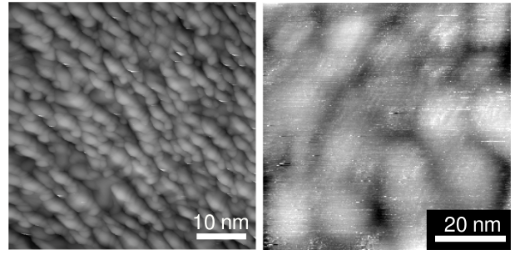
\includegraphics[width=.45\linewidth]{/Users/pascu/Desktop/C-Kurs/praktikum4/p422/assets/3_goldkugel/Gold_vergleich.png}
    \caption{Proben werden gezeigt. links: Gold auf Silizium(das Beobachtete), rechts: Gold auf Saphir}
    \label{fig:goldkugel_vergleich}
  \end{figure}

\newpage
\section{HOPG-Probe}
Als nächstes soll eine der HOPG-Proben (wir verwendeten Nummer 17) beobachtet werden. 
Optische Bilder der verwendeten Spitze und des TEM-Netzes sind in Abb. \ref{fig:spitze-2} und \ref{fig:gitter-hopg} gezeigt.


Graphit besteht aus Schichten, welche untereinander nur schwach durch Van-der-Waals-Bindungen
zusammengehalten werden. Darum kann eine obere Schicht mithilfe eines Stücks Klebeband abgezogen werden.
Dies tun wir hier, um eine möglichst wenig verunreinigte Probe zu erhalten. Die Probe vor dem
Abziehen ist in Abb. \ref{fig:hopg-raw-lupe} und nach mehrfachem Abziehen in Abb. \ref{fig:hopg-nach-lupe}
gezeigt. Im optischen Bild ist kein großer Unterschied zu erkennen, da nur wenige Atomschichten entfernt wurden.



Zunächst wird ein Testlauf im Constant Current Modus durchgeführt, um sicherzugehen, dass
es im betrachteten Ausschnitt keine größeren Stufen gibt.
Anschließend wird zum Constant Height Modus gewechselt, indem der P-Parameter auf $0$ und der
I-Parameter auf einen sehr niedrigen Wert ($4 - 10$) gesetzt werden.

Für die erste Abbildung wird mit einem verglichen zur Atomgröße relativ großen Bildausschnitt von $\SI{12.5}{\nm}$ begonnen (Abb. \ref{fig:hopg-large}). Hier lassen sich bereits regelmäßige Strukturen erkennen.


Nach Anpassung einiger Parameter gelingt es schließlich auch, auf kleineren Skalen gute Bilder zu erhalten, siehe Abb. \ref{fig:hopg-medium} und \ref{fig:hopg-small}



\begin{table}[h]
    \centering
    \begin{tabular}{c||c|c|c|c|c}
        Linie Nr. & $\phi/\si{\deg}$ & $R/\si{\nm}$ & $n$ & $a/\si{\nm}$ & $\Delta a/\si{\nm}$ \\
        \hline
        $1$ & $17.0 $   & $1.280$ & $5$ & $0.256$ & $0.010$ \\
        $2$ & $-49.0$	& $0.642$ & $3$ & $0.214$ & $0.017$ \\
        $3$ & $16.4	$   & $1.279$ & $5$ & $0.256$ & $0.010$ \\
        $4$ & $-50.9$	& $0.636$ & $3$ & $0.212$ & $0.017$
    \end{tabular}
    \caption{gemessene Längen und Winkel im HOPG. $\Delta\phi=\ang{3.0}$, $\Delta R = \SI{0.050}{\nm}$. $\phi$ ist der Winkel der Linie zur Horizontalen, R die Länge der Linie und $n$ steht für die Anzahl an Gitterabständen, welche die Linie überspannt. Die Nummerierung der Linien kommt aus Abb. \ref{fig:hopg-medium} (1 und 3 sind die längeren, 2 und 4 die kürzeren Linien).}
    \label{tab:hopg-daten-1}
\end{table}



\clearpage
\section{Fazit}
Die Funktionsweise und den Einsatz eines Rastertunnelmikroskops (RTM) wurde während des Versuchs erfolgreich untersucht. Es wurden Goldproben analysiert, wobei die erwarteten Aufnahmen erzielt wurden, die den theoretischen Vorhersagen entsprachen. Die Oberflächenbehandlung der Proben führte zur Beobachtung wolkenähnlicher Strukturen, wie prognostiziert. 

Außerdem wurden mögliche Ursachen für Bildfehler untersucht, darunter die Präparation der Probe, die Empfindlichkeit der Geräte und äußere Störeinflüsse. Diese Analyse lieferte wertvolle Einblicke in die Herausforderungen und die Präzisionsanforderungen bei der Bildgebung mit dem RTM.







\clearpage
\section{Anhang}


\clearpage
\begin{thebibliography}{9}

\bibitem{Anleitung}
\textit{Physikalisches Praktikum Teil IV -- Versuchsbeschreibungen}, Universität Bonn, 10.10.2024

\bibitem{wiki-stm}

\bibitem{meshsize}
\todo{Was Sie über TEM-Grids wissen sollten}, Science Services, Abruf 29.11.2024

\bibitem{graphite}
\textit{Graphite}, mindat.org, Abruf 29.11.2024, https://www.mindat.org/min-1740.html

\bibitem{feinstaub}
\textit{Feinstaub}, Chemie.de, Abruf 24.11.2024, \url{https://www.chemie.de/lexikon/Feinstaub.html}


\end{thebibliography}

\end{document}

